\documentclass[12pt]{report}

\usepackage{setspace}
\usepackage{bm}
\usepackage{gensymb}
\usepackage{graphicx}
\usepackage{float}

\graphicspath{{figs/}}

%%%%%%%%%%%%%%%%%%%%%%%%%%%%%%%%%
% PACKAGE IMPORTS
%%%%%%%%%%%%%%%%%%%%%%%%%%%%%%%%%


\usepackage[tmargin=2cm,rmargin=1in,lmargin=1in,margin=0.85in,bmargin=2cm,footskip=.2in]{geometry}
\usepackage{amsmath,amsfonts,amsthm,amssymb,mathtools}
\usepackage[varbb]{newpxmath}
\usepackage{xfrac}
\usepackage[makeroom]{cancel}
\usepackage{mathtools}
\usepackage{bookmark}
\usepackage{enumitem}
\usepackage{hyperref,theoremref}
\hypersetup{
	pdftitle={Assignment},
	colorlinks=true, linkcolor=doc!90,
	bookmarksnumbered=true,
	bookmarksopen=true
}
\usepackage[most,many,breakable]{tcolorbox}
\usepackage{xcolor}
\usepackage{varwidth}
\usepackage{varwidth}
\usepackage{etoolbox}
%\usepackage{authblk}
\usepackage{nameref}
\usepackage{multicol,array}
\usepackage{tikz-cd}
\usepackage[ruled,vlined,linesnumbered]{algorithm2e}
\usepackage{comment} % enables the use of multi-line comments (\ifx \fi) 
\usepackage{import}
\usepackage{xifthen}
\usepackage{pdfpages}
\usepackage{transparent}

\newcommand\mycommfont[1]{\footnotesize\ttfamily\textcolor{blue}{#1}}
\SetCommentSty{mycommfont}
\newcommand{\incfig}[1]{%
    \def\svgwidth{\columnwidth}
    \import{./figures/}{#1.pdf_tex}
}

\usepackage{tikzsymbols}
\renewcommand\qedsymbol{$\Laughey$}


%\usepackage{import}
%\usepackage{xifthen}
%\usepackage{pdfpages}
%\usepackage{transparent}


%%%%%%%%%%%%%%%%%%%%%%%%%%%%%%
% SELF MADE COLORS
%%%%%%%%%%%%%%%%%%%%%%%%%%%%%%



\definecolor{myg}{RGB}{56, 140, 70}
\definecolor{myb}{RGB}{45, 111, 177}
\definecolor{myr}{RGB}{199, 68, 64}
\definecolor{mytheorembg}{HTML}{F2F2F9}
\definecolor{mytheoremfr}{HTML}{00007B}
\definecolor{mylenmabg}{HTML}{FFFAF8}
\definecolor{mylenmafr}{HTML}{983b0f}
\definecolor{mypropbg}{HTML}{f2fbfc}
\definecolor{mypropfr}{HTML}{191971}
\definecolor{myexamplebg}{HTML}{F2FBF8}
\definecolor{myexamplefr}{HTML}{88D6D1}
\definecolor{myexampleti}{HTML}{2A7F7F}
\definecolor{mydefinitbg}{HTML}{E5E5FF}
\definecolor{mydefinitfr}{HTML}{3F3FA3}
\definecolor{notesgreen}{RGB}{0,162,0}
\definecolor{myp}{RGB}{197, 92, 212}
\definecolor{mygr}{HTML}{2C3338}
\definecolor{myred}{RGB}{127,0,0}
\definecolor{myyellow}{RGB}{169,121,69}
\definecolor{myexercisebg}{HTML}{F2FBF8}
\definecolor{myexercisefg}{HTML}{88D6D1}


%%%%%%%%%%%%%%%%%%%%%%%%%%%%
% TCOLORBOX SETUPS
%%%%%%%%%%%%%%%%%%%%%%%%%%%%

\setlength{\parindent}{1cm}
%================================
% THEOREM BOX
%================================

\tcbuselibrary{theorems,skins,hooks}
\newtcbtheorem[number within=section]{Theorem}{Theorem}
{%
	enhanced,
	breakable,
	colback = mytheorembg,
	frame hidden,
	boxrule = 0sp,
	borderline west = {2pt}{0pt}{mytheoremfr},
	sharp corners,
	detach title,
	before upper = \tcbtitle\par\smallskip,
	coltitle = mytheoremfr,
	fonttitle = \bfseries\sffamily,
	description font = \mdseries,
	separator sign none,
	segmentation style={solid, mytheoremfr},
}
{th}

\tcbuselibrary{theorems,skins,hooks}
\newtcbtheorem[number within=chapter]{theorem}{Theorem}
{%
	enhanced,
	breakable,
	colback = mytheorembg,
	frame hidden,
	boxrule = 0sp,
	borderline west = {2pt}{0pt}{mytheoremfr},
	sharp corners,
	detach title,
	before upper = \tcbtitle\par\smallskip,
	coltitle = mytheoremfr,
	fonttitle = \bfseries\sffamily,
	description font = \mdseries,
	separator sign none,
	segmentation style={solid, mytheoremfr},
}
{th}


\tcbuselibrary{theorems,skins,hooks}
\newtcolorbox{Theoremcon}
{%
	enhanced
	,breakable
	,colback = mytheorembg
	,frame hidden
	,boxrule = 0sp
	,borderline west = {2pt}{0pt}{mytheoremfr}
	,sharp corners
	,description font = \mdseries
	,separator sign none
}

%================================
% Corollery
%================================
\tcbuselibrary{theorems,skins,hooks}
\newtcbtheorem[number within=section]{Corollary}{Corollary}
{%
	enhanced
	,breakable
	,colback = myp!10
	,frame hidden
	,boxrule = 0sp
	,borderline west = {2pt}{0pt}{myp!85!black}
	,sharp corners
	,detach title
	,before upper = \tcbtitle\par\smallskip
	,coltitle = myp!85!black
	,fonttitle = \bfseries\sffamily
	,description font = \mdseries
	,separator sign none
	,segmentation style={solid, myp!85!black}
}
{th}
\tcbuselibrary{theorems,skins,hooks}
\newtcbtheorem[number within=chapter]{corollary}{Corollary}
{%
	enhanced
	,breakable
	,colback = myp!10
	,frame hidden
	,boxrule = 0sp
	,borderline west = {2pt}{0pt}{myp!85!black}
	,sharp corners
	,detach title
	,before upper = \tcbtitle\par\smallskip
	,coltitle = myp!85!black
	,fonttitle = \bfseries\sffamily
	,description font = \mdseries
	,separator sign none
	,segmentation style={solid, myp!85!black}
}
{th}


%================================
% LENMA
%================================

\tcbuselibrary{theorems,skins,hooks}
\newtcbtheorem[number within=section]{Lenma}{Lenma}
{%
	enhanced,
	breakable,
	colback = mylenmabg,
	frame hidden,
	boxrule = 0sp,
	borderline west = {2pt}{0pt}{mylenmafr},
	sharp corners,
	detach title,
	before upper = \tcbtitle\par\smallskip,
	coltitle = mylenmafr,
	fonttitle = \bfseries\sffamily,
	description font = \mdseries,
	separator sign none,
	segmentation style={solid, mylenmafr},
}
{th}

\tcbuselibrary{theorems,skins,hooks}
\newtcbtheorem[number within=chapter]{lenma}{Lenma}
{%
	enhanced,
	breakable,
	colback = mylenmabg,
	frame hidden,
	boxrule = 0sp,
	borderline west = {2pt}{0pt}{mylenmafr},
	sharp corners,
	detach title,
	before upper = \tcbtitle\par\smallskip,
	coltitle = mylenmafr,
	fonttitle = \bfseries\sffamily,
	description font = \mdseries,
	separator sign none,
	segmentation style={solid, mylenmafr},
}
{th}


%================================
% PROPOSITION
%================================

\tcbuselibrary{theorems,skins,hooks}
\newtcbtheorem[number within=section]{Prop}{Proposition}
{%
	enhanced,
	breakable,
	colback = mypropbg,
	frame hidden,
	boxrule = 0sp,
	borderline west = {2pt}{0pt}{mypropfr},
	sharp corners,
	detach title,
	before upper = \tcbtitle\par\smallskip,
	coltitle = mypropfr,
	fonttitle = \bfseries\sffamily,
	description font = \mdseries,
	separator sign none,
	segmentation style={solid, mypropfr},
}
{th}

\tcbuselibrary{theorems,skins,hooks}
\newtcbtheorem[number within=chapter]{prop}{Proposition}
{%
	enhanced,
	breakable,
	colback = mypropbg,
	frame hidden,
	boxrule = 0sp,
	borderline west = {2pt}{0pt}{mypropfr},
	sharp corners,
	detach title,
	before upper = \tcbtitle\par\smallskip,
	coltitle = mypropfr,
	fonttitle = \bfseries\sffamily,
	description font = \mdseries,
	separator sign none,
	segmentation style={solid, mypropfr},
}
{th}


%================================
% CLAIM
%================================

\tcbuselibrary{theorems,skins,hooks}
\newtcbtheorem[number within=section]{claim}{Claim}
{%
	enhanced
	,breakable
	,colback = myg!10
	,frame hidden
	,boxrule = 0sp
	,borderline west = {2pt}{0pt}{myg}
	,sharp corners
	,detach title
	,before upper = \tcbtitle\par\smallskip
	,coltitle = myg!85!black
	,fonttitle = \bfseries\sffamily
	,description font = \mdseries
	,separator sign none
	,segmentation style={solid, myg!85!black}
}
{th}



%================================
% Exercise
%================================

\tcbuselibrary{theorems,skins,hooks}
\newtcbtheorem[number within=section]{Exercise}{Exercise}
{%
	enhanced,
	breakable,
	colback = myexercisebg,
	frame hidden,
	boxrule = 0sp,
	borderline west = {2pt}{0pt}{myexercisefg},
	sharp corners,
	detach title,
	before upper = \tcbtitle\par\smallskip,
	coltitle = myexercisefg,
	fonttitle = \bfseries\sffamily,
	description font = \mdseries,
	separator sign none,
	segmentation style={solid, myexercisefg},
}
{th}

\tcbuselibrary{theorems,skins,hooks}
\newtcbtheorem[number within=chapter]{exercise}{Exercise}
{%
	enhanced,
	breakable,
	colback = myexercisebg,
	frame hidden,
	boxrule = 0sp,
	borderline west = {2pt}{0pt}{myexercisefg},
	sharp corners,
	detach title,
	before upper = \tcbtitle\par\smallskip,
	coltitle = myexercisefg,
	fonttitle = \bfseries\sffamily,
	description font = \mdseries,
	separator sign none,
	segmentation style={solid, myexercisefg},
}
{th}

%================================
% EXAMPLE BOX
%================================

\newtcbtheorem[number within=section]{Example}{Example}
{%
	colback = myexamplebg
	,breakable
	,colframe = myexamplefr
	,coltitle = myexampleti
	,boxrule = 1pt
	,sharp corners
	,detach title
	,before upper=\tcbtitle\par\smallskip
	,fonttitle = \bfseries
	,description font = \mdseries
	,separator sign none
	,description delimiters parenthesis
}
{ex}

\newtcbtheorem[number within=chapter]{example}{Example}
{%
	colback = myexamplebg
	,breakable
	,colframe = myexamplefr
	,coltitle = myexampleti
	,boxrule = 1pt
	,sharp corners
	,detach title
	,before upper=\tcbtitle\par\smallskip
	,fonttitle = \bfseries
	,description font = \mdseries
	,separator sign none
	,description delimiters parenthesis
}
{ex}

%================================
% DEFINITION BOX
%================================

\newtcbtheorem[number within=section]{Definition}{Definition}{enhanced,
	before skip=2mm,after skip=2mm, colback=red!5,colframe=red!80!black,boxrule=0.5mm,
	attach boxed title to top left={xshift=1cm,yshift*=1mm-\tcboxedtitleheight}, varwidth boxed title*=-3cm,
	boxed title style={frame code={
					\path[fill=tcbcolback]
					([yshift=-1mm,xshift=-1mm]frame.north west)
					arc[start angle=0,end angle=180,radius=1mm]
					([yshift=-1mm,xshift=1mm]frame.north east)
					arc[start angle=180,end angle=0,radius=1mm];
					\path[left color=tcbcolback!60!black,right color=tcbcolback!60!black,
						middle color=tcbcolback!80!black]
					([xshift=-2mm]frame.north west) -- ([xshift=2mm]frame.north east)
					[rounded corners=1mm]-- ([xshift=1mm,yshift=-1mm]frame.north east)
					-- (frame.south east) -- (frame.south west)
					-- ([xshift=-1mm,yshift=-1mm]frame.north west)
					[sharp corners]-- cycle;
				},interior engine=empty,
		},
	fonttitle=\bfseries,
	title={#2},#1}{def}
\newtcbtheorem[number within=chapter]{definition}{Definition}{enhanced,
	before skip=2mm,after skip=2mm, colback=red!5,colframe=red!80!black,boxrule=0.5mm,
	attach boxed title to top left={xshift=1cm,yshift*=1mm-\tcboxedtitleheight}, varwidth boxed title*=-3cm,
	boxed title style={frame code={
					\path[fill=tcbcolback]
					([yshift=-1mm,xshift=-1mm]frame.north west)
					arc[start angle=0,end angle=180,radius=1mm]
					([yshift=-1mm,xshift=1mm]frame.north east)
					arc[start angle=180,end angle=0,radius=1mm];
					\path[left color=tcbcolback!60!black,right color=tcbcolback!60!black,
						middle color=tcbcolback!80!black]
					([xshift=-2mm]frame.north west) -- ([xshift=2mm]frame.north east)
					[rounded corners=1mm]-- ([xshift=1mm,yshift=-1mm]frame.north east)
					-- (frame.south east) -- (frame.south west)
					-- ([xshift=-1mm,yshift=-1mm]frame.north west)
					[sharp corners]-- cycle;
				},interior engine=empty,
		},
	fonttitle=\bfseries,
	title={#2},#1}{def}



%================================
% Solution BOX
%================================

\makeatletter
\newtcbtheorem{question}{Question}{enhanced,
	breakable,
	colback=white,
	colframe=myb!80!black,
	attach boxed title to top left={yshift*=-\tcboxedtitleheight},
	fonttitle=\bfseries,
	title={#2},
	boxed title size=title,
	boxed title style={%
			sharp corners,
			rounded corners=northwest,
			colback=tcbcolframe,
			boxrule=0pt,
		},
	underlay boxed title={%
			\path[fill=tcbcolframe] (title.south west)--(title.south east)
			to[out=0, in=180] ([xshift=5mm]title.east)--
			(title.center-|frame.east)
			[rounded corners=\kvtcb@arc] |-
			(frame.north) -| cycle;
		},
	#1
}{def}
\makeatother

%================================
% SOLUTION BOX
%================================

\makeatletter
\newtcolorbox{solutions}{enhanced,
	breakable,
	colback=white,
	colframe=myg!80!black,
	attach boxed title to top left={yshift*=-\tcboxedtitleheight},
	title=Solution,
	boxed title size=title,
	boxed title style={%
			sharp corners,
			rounded corners=northwest,
			colback=tcbcolframe,
			boxrule=0pt,
		},
	underlay boxed title={%
			\path[fill=tcbcolframe] (title.south west)--(title.south east)
			to[out=0, in=180] ([xshift=5mm]title.east)--
			(title.center-|frame.east)
			[rounded corners=\kvtcb@arc] |-
			(frame.north) -| cycle;
		},
}
\makeatother

%================================
% Question BOX
%================================

\makeatletter
\newtcbtheorem{qstion}{Question}{enhanced,
	breakable,
	colback=white,
	colframe=mygr,
	attach boxed title to top left={yshift*=-\tcboxedtitleheight},
	fonttitle=\bfseries,
	title={#2},
	boxed title size=title,
	boxed title style={%
			sharp corners,
			rounded corners=northwest,
			colback=tcbcolframe,
			boxrule=0pt,
		},
	underlay boxed title={%
			\path[fill=tcbcolframe] (title.south west)--(title.south east)
			to[out=0, in=180] ([xshift=5mm]title.east)--
			(title.center-|frame.east)
			[rounded corners=\kvtcb@arc] |-
			(frame.north) -| cycle;
		},
	#1
}{def}
\makeatother

\newtcbtheorem[number within=chapter]{wconc}{Wrong Concept}{
	breakable,
	enhanced,
	colback=white,
	colframe=myr,
	arc=0pt,
	outer arc=0pt,
	fonttitle=\bfseries\sffamily\large,
	colbacktitle=myr,
	attach boxed title to top left={},
	boxed title style={
			enhanced,
			skin=enhancedfirst jigsaw,
			arc=3pt,
			bottom=0pt,
			interior style={fill=myr}
		},
	#1
}{def}



%================================
% NOTE BOX
%================================

\usetikzlibrary{arrows,calc,shadows.blur}
\tcbuselibrary{skins}
\newtcolorbox{note}[1][]{%
	enhanced jigsaw,
	colback=gray!20!white,%
	colframe=gray!80!black,
	size=small,
	boxrule=1pt,
	title=\textbf{Note:-},
	halign title=flush center,
	coltitle=black,
	breakable,
	drop shadow=black!50!white,
	attach boxed title to top left={xshift=1cm,yshift=-\tcboxedtitleheight/2,yshifttext=-\tcboxedtitleheight/2},
	minipage boxed title=1.5cm,
	boxed title style={%
			colback=white,
			size=fbox,
			boxrule=1pt,
			boxsep=2pt,
			underlay={%
					\coordinate (dotA) at ($(interior.west) + (-0.5pt,0)$);
					\coordinate (dotB) at ($(interior.east) + (0.5pt,0)$);
					\begin{scope}
						\clip (interior.north west) rectangle ([xshift=3ex]interior.east);
						\filldraw [white, blur shadow={shadow opacity=60, shadow yshift=-.75ex}, rounded corners=2pt] (interior.north west) rectangle (interior.south east);
					\end{scope}
					\begin{scope}[gray!80!black]
						\fill (dotA) circle (2pt);
						\fill (dotB) circle (2pt);
					\end{scope}
				},
		},
	#1,
}

%================================
% Solution BOX
%================================

\makeatletter
\newtcbtheorem{solution}{Solution}{enhanced,
	breakable,
	colback=white,
	colframe=myg!80!black,
	attach boxed title to top left={yshift*=-\tcboxedtitleheight},
	fonttitle=\bfseries,
	title={#2},
	boxed title size=title,
	boxed title style={%
			sharp corners,
			rounded corners=northwest,
			colback=tcbcolframe,
			boxrule=0pt,
		},
	underlay boxed title={%
			\path[fill=tcbcolframe] (title.south west)--(title.south east)
			to[out=0, in=180] ([xshift=5mm]title.east)--
			(title.center-|frame.east)
			[rounded corners=\kvtcb@arc] |-
			(frame.north) -| cycle;
		},
	#1
}{def}
\makeatother

%%%%%%%%%%%%%%%%%%%%%%%%%%%%%%
% SELF MADE COMMANDS
%%%%%%%%%%%%%%%%%%%%%%%%%%%%%%


\newcommand{\thm}[2]{\begin{Theorem}{#1}{}#2\end{Theorem}}
\newcommand{\cor}[2]{\begin{Corollary}{#1}{}#2\end{Corollary}}
\newcommand{\mlenma}[2]{\begin{Lenma}{#1}{}#2\end{Lenma}}
\newcommand{\mprop}[2]{\begin{Prop}{#1}{}#2\end{Prop}}
\newcommand{\clm}[3]{\begin{claim}{#1}{#2}#3\end{claim}}
\newcommand{\wc}[2]{\begin{wconc}{#1}{}\setlength{\parindent}{1cm}#2\end{wconc}}
\newcommand{\thmcon}[1]{\begin{Theoremcon}{#1}\end{Theoremcon}}
\newcommand{\ex}[2]{\begin{Example}{#1}{}#2\end{Example}}
\newcommand{\dfn}[2]{\begin{Definition}[colbacktitle=red!75!black]{#1}{}#2\end{Definition}}
\newcommand{\dfnc}[2]{\begin{definition}[colbacktitle=red!75!black]{#1}{}#2\end{definition}}
\newcommand{\qs}[2]{\begin{question}{#1}{}#2\end{question}}
\newcommand{\pf}[2]{\begin{myproof}[#1]#2\end{myproof}}
\newcommand{\nt}[1]{\begin{note}#1\end{note}}

\newcommand{\as}[2]{\begin{solution}{#1}{}#2\end{solution}}

\newcommand*\circled[1]{\tikz[baseline=(char.base)]{
		\node[shape=circle,draw,inner sep=1pt] (char) {#1};}}
\newcommand\getcurrentref[1]{%
	\ifnumequal{\value{#1}}{0}
	{??}
	{\the\value{#1}}%
}
\newcommand{\getCurrentSectionNumber}{\getcurrentref{section}}
\newenvironment{myproof}[1][\proofname]{%
	\proof[\bfseries #1: ]%
}{\endproof}

\newcommand{\mclm}[2]{\begin{myclaim}[#1]#2\end{myclaim}}
\newenvironment{myclaim}[1][\claimname]{\proof[\bfseries #1: ]}{}

\newcounter{mylabelcounter}

\makeatletter
\newcommand{\setword}[2]{%
	\phantomsection
	#1\def\@currentlabel{\unexpanded{#1}}\label{#2}%
}
\makeatother




\tikzset{
	symbol/.style={
			draw=none,
			every to/.append style={
					edge node={node [sloped, allow upside down, auto=false]{$#1$}}}
		}
}


% deliminators
\DeclarePairedDelimiter{\abs}{\lvert}{\rvert}
\DeclarePairedDelimiter{\norm}{\lVert}{\rVert}

\DeclarePairedDelimiter{\ceil}{\lceil}{\rceil}
\DeclarePairedDelimiter{\floor}{\lfloor}{\rfloor}
\DeclarePairedDelimiter{\round}{\lfloor}{\rceil}

\newsavebox\diffdbox
\newcommand{\slantedromand}{{\mathpalette\makesl{d}}}
\newcommand{\makesl}[2]{%
\begingroup
\sbox{\diffdbox}{$\mathsurround=0pt#1\mathrm{#2}$}%
\pdfsave
\pdfsetmatrix{1 0 0.2 1}%
\rlap{\usebox{\diffdbox}}%
\pdfrestore
\hskip\wd\diffdbox
\endgroup
}
\newcommand{\dd}[1][]{\ensuremath{\mathop{}\!\ifstrempty{#1}{%
\slantedromand\@ifnextchar^{\hspace{0.2ex}}{\hspace{0.1ex}}}%
{\slantedromand\hspace{0.2ex}^{#1}}}}
\ProvideDocumentCommand\dv{o m g}{%
  \ensuremath{%
    \IfValueTF{#3}{%
      \IfNoValueTF{#1}{%
        \frac{\dd #2}{\dd #3}%
      }{%
        \frac{\dd^{#1} #2}{\dd #3^{#1}}%
      }%
    }{%
      \IfNoValueTF{#1}{%
        \frac{\dd}{\dd #2}%
      }{%
        \frac{\dd^{#1}}{\dd #2^{#1}}%
      }%
    }%
  }%
}
\providecommand*{\pdv}[3][]{\frac{\partial^{#1}#2}{\partial#3^{#1}}}
%  - others
\DeclareMathOperator{\Lap}{\mathcal{L}}
\DeclareMathOperator{\Var}{Var} % varience
\DeclareMathOperator{\Cov}{Cov} % covarience
\DeclareMathOperator{\E}{E} % expected

% Since the amsthm package isn't loaded

% I prefer the slanted \leq
\let\oldleq\leq % save them in case they're every wanted
\let\oldgeq\geq
\renewcommand{\leq}{\leqslant}
\renewcommand{\geq}{\geqslant}

% % redefine matrix env to allow for alignment, use r as default
% \renewcommand*\env@matrix[1][r]{\hskip -\arraycolsep
%     \let\@ifnextchar\new@ifnextchar
%     \array{*\c@MaxMatrixCols #1}}


%\usepackage{framed}
%\usepackage{titletoc}
%\usepackage{etoolbox}
%\usepackage{lmodern}


%\patchcmd{\tableofcontents}{\contentsname}{\sffamily\contentsname}{}{}

%\renewenvironment{leftbar}
%{\def\FrameCommand{\hspace{6em}%
%		{\color{myyellow}\vrule width 2pt depth 6pt}\hspace{1em}}%
%	\MakeFramed{\parshape 1 0cm \dimexpr\textwidth-6em\relax\FrameRestore}\vskip2pt%
%}
%{\endMakeFramed}

%\titlecontents{chapter}
%[0em]{\vspace*{2\baselineskip}}
%{\parbox{4.5em}{%
%		\hfill\Huge\sffamily\bfseries\color{myred}\thecontentspage}%
%	\vspace*{-2.3\baselineskip}\leftbar\textsc{\small\chaptername~\thecontentslabel}\\\sffamily}
%{}{\endleftbar}
%\titlecontents{section}
%[8.4em]
%{\sffamily\contentslabel{3em}}{}{}
%{\hspace{0.5em}\nobreak\itshape\color{myred}\contentspage}
%\titlecontents{subsection}
%[8.4em]
%{\sffamily\contentslabel{3em}}{}{}  
%{\hspace{0.5em}\nobreak\itshape\color{myred}\contentspage}



%%%%%%%%%%%%%%%%%%%%%%%%%%%%%%%%%%%%%%%%%%%
% TABLE OF CONTENTS
%%%%%%%%%%%%%%%%%%%%%%%%%%%%%%%%%%%%%%%%%%%

\usepackage{tikz}
\definecolor{doc}{RGB}{0,60,110}
\usepackage{titletoc}
\contentsmargin{0cm}
\titlecontents{chapter}[3.7pc]
{\addvspace{30pt}%
	\begin{tikzpicture}[remember picture, overlay]%
		\draw[fill=doc!60,draw=doc!60] (-7,-.1) rectangle (-0.9,.5);%
		\pgftext[left,x=-3.5cm,y=0.2cm]{\color{white}\Large\sc\bfseries Chapter\ \thecontentslabel};%
	\end{tikzpicture}\color{doc!60}\large\sc\bfseries}%
{}
{}
{\;\titlerule\;\large\sc\bfseries Page \thecontentspage
	\begin{tikzpicture}[remember picture, overlay]
		\draw[fill=doc!60,draw=doc!60] (2pt,0) rectangle (4,0.1pt);
	\end{tikzpicture}}%
\titlecontents{section}[3.7pc]
{\addvspace{2pt}}
{\contentslabel[\thecontentslabel]{2pc}}
{}
{\hfill\small \thecontentspage}
[]
\titlecontents*{subsection}[3.7pc]
{\addvspace{-1pt}\small}
{}
{}
{\ --- \small\thecontentspage}
[ \textbullet\ ][]

\makeatletter
\renewcommand{\tableofcontents}{%
	\chapter*{%
	  \vspace*{-20\p@}%
	  \begin{tikzpicture}[remember picture, overlay]%
		  \pgftext[right,x=15cm,y=0.2cm]{\color{doc!60}\Huge\sc\bfseries \contentsname};%
		  \draw[fill=doc!60,draw=doc!60] (13,-.75) rectangle (20,1);%
		  \clip (13,-.75) rectangle (20,1);
		  \pgftext[right,x=15cm,y=0.2cm]{\color{white}\Huge\sc\bfseries \contentsname};%
	  \end{tikzpicture}}%
	\@starttoc{toc}}
\makeatother


%From M275 "Topology" at SJSU
\newcommand{\id}{\mathrm{id}}
\newcommand{\taking}[1]{\xrightarrow{#1}}
\newcommand{\inv}{^{-1}}

%From M170 "Introduction to Graph Theory" at SJSU
\DeclareMathOperator{\diam}{diam}
\DeclareMathOperator{\ord}{ord}
\newcommand{\defeq}{\overset{\mathrm{def}}{=}}

%From the USAMO .tex files
\newcommand{\ts}{\textsuperscript}
\newcommand{\dg}{^\circ}
\newcommand{\ii}{\item}

% % From Math 55 and Math 145 at Harvard
% \newenvironment{subproof}[1][Proof]{%
% \begin{proof}[#1] \renewcommand{\qedsymbol}{$\blacksquare$}}%
% {\end{proof}}

\newcommand{\liff}{\leftrightarrow}
\newcommand{\lthen}{\rightarrow}
\newcommand{\opname}{\operatorname}
\newcommand{\surjto}{\twoheadrightarrow}
\newcommand{\injto}{\hookrightarrow}
\newcommand{\On}{\mathrm{On}} % ordinals
\DeclareMathOperator{\img}{im} % Image
\DeclareMathOperator{\Img}{Im} % Image
\DeclareMathOperator{\coker}{coker} % Cokernel
\DeclareMathOperator{\Coker}{Coker} % Cokernel
\DeclareMathOperator{\Ker}{Ker} % Kernel
\DeclareMathOperator{\rank}{rank}
\DeclareMathOperator{\Spec}{Spec} % spectrum
\DeclareMathOperator{\Tr}{Tr} % trace
\DeclareMathOperator{\pr}{pr} % projection
\DeclareMathOperator{\ext}{ext} % extension
\DeclareMathOperator{\pred}{pred} % predecessor
\DeclareMathOperator{\dom}{dom} % domain
\DeclareMathOperator{\ran}{ran} % range
\DeclareMathOperator{\Hom}{Hom} % homomorphism
\DeclareMathOperator{\Mor}{Mor} % morphisms
\DeclareMathOperator{\End}{End} % endomorphism

\newcommand{\eps}{\epsilon}
\newcommand{\veps}{\varepsilon}
\newcommand{\ol}{\overline}
\newcommand{\ul}{\underline}
\newcommand{\wt}{\widetilde}
\newcommand{\wh}{\widehat}
\newcommand{\vocab}[1]{\textbf{\color{blue} #1}}
\providecommand{\half}{\frac{1}{2}}
\newcommand{\dang}{\measuredangle} %% Directed angle
\newcommand{\ray}[1]{\overrightarrow{#1}}
\newcommand{\seg}[1]{\overline{#1}}
\newcommand{\arc}[1]{\wideparen{#1}}
\DeclareMathOperator{\cis}{cis}
\DeclareMathOperator*{\lcm}{lcm}
\DeclareMathOperator*{\argmin}{arg min}
\DeclareMathOperator*{\argmax}{arg max}
\newcommand{\cycsum}{\sum_{\mathrm{cyc}}}
\newcommand{\symsum}{\sum_{\mathrm{sym}}}
\newcommand{\cycprod}{\prod_{\mathrm{cyc}}}
\newcommand{\symprod}{\prod_{\mathrm{sym}}}
\newcommand{\Qed}{\begin{flushright}\qed\end{flushright}}
\newcommand{\parinn}{\setlength{\parindent}{1cm}}
\newcommand{\parinf}{\setlength{\parindent}{0cm}}
% \newcommand{\norm}{\|\cdot\|}
\newcommand{\inorm}{\norm_{\infty}}
\newcommand{\opensets}{\{V_{\alpha}\}_{\alpha\in I}}
\newcommand{\oset}{V_{\alpha}}
\newcommand{\opset}[1]{V_{\alpha_{#1}}}
\newcommand{\lub}{\text{lub}}
\newcommand{\del}[2]{\frac{\partial #1}{\partial #2}}
\newcommand{\Del}[3]{\frac{\partial^{#1} #2}{\partial^{#1} #3}}
\newcommand{\deld}[2]{\dfrac{\partial #1}{\partial #2}}
\newcommand{\Deld}[3]{\dfrac{\partial^{#1} #2}{\partial^{#1} #3}}
\newcommand{\lm}{\lambda}
\newcommand{\uin}{\mathbin{\rotatebox[origin=c]{90}{$\in$}}}
\newcommand{\usubset}{\mathbin{\rotatebox[origin=c]{90}{$\subset$}}}
\newcommand{\lt}{\left}
\newcommand{\rt}{\right}
\newcommand{\bs}[1]{\boldsymbol{#1}}
\newcommand{\exs}{\exists}
\newcommand{\st}{\strut}
\newcommand{\dps}[1]{\displaystyle{#1}}

\newcommand{\sol}{\setlength{\parindent}{0cm}\textbf{\textit{Solution:}}\setlength{\parindent}{1cm} }
\newcommand{\solve}[1]{\setlength{\parindent}{0cm}\textbf{\textit{Solution: }}\setlength{\parindent}{1cm}#1 \Qed}

% Things Lie
\newcommand{\kb}{\mathfrak b}
\newcommand{\kg}{\mathfrak g}
\newcommand{\kh}{\mathfrak h}
\newcommand{\kn}{\mathfrak n}
\newcommand{\ku}{\mathfrak u}
\newcommand{\kz}{\mathfrak z}
\DeclareMathOperator{\Ext}{Ext} % Ext functor
\DeclareMathOperator{\Tor}{Tor} % Tor functor
\newcommand{\gl}{\opname{\mathfrak{gl}}} % frak gl group
\renewcommand{\sl}{\opname{\mathfrak{sl}}} % frak sl group chktex 6

% More script letters etc.
\newcommand{\SA}{\mathcal A}
\newcommand{\SB}{\mathcal B}
\newcommand{\SC}{\mathcal C}
\newcommand{\SF}{\mathcal F}
\newcommand{\SG}{\mathcal G}
\newcommand{\SH}{\mathcal H}
\newcommand{\OO}{\mathcal O}

\newcommand{\SCA}{\mathscr A}
\newcommand{\SCB}{\mathscr B}
\newcommand{\SCC}{\mathscr C}
\newcommand{\SCD}{\mathscr D}
\newcommand{\SCE}{\mathscr E}
\newcommand{\SCF}{\mathscr F}
\newcommand{\SCG}{\mathscr G}
\newcommand{\SCH}{\mathscr H}

% Mathfrak primes
\newcommand{\km}{\mathfrak m}
\newcommand{\kp}{\mathfrak p}
\newcommand{\kq}{\mathfrak q}

% number sets
\newcommand{\RR}[1][]{\ensuremath{\ifstrempty{#1}{\mathbb{R}}{\mathbb{R}^{#1}}}}
\newcommand{\NN}[1][]{\ensuremath{\ifstrempty{#1}{\mathbb{N}}{\mathbb{N}^{#1}}}}
\newcommand{\ZZ}[1][]{\ensuremath{\ifstrempty{#1}{\mathbb{Z}}{\mathbb{Z}^{#1}}}}
\newcommand{\QQ}[1][]{\ensuremath{\ifstrempty{#1}{\mathbb{Q}}{\mathbb{Q}^{#1}}}}
\newcommand{\CC}[1][]{\ensuremath{\ifstrempty{#1}{\mathbb{C}}{\mathbb{C}^{#1}}}}
\newcommand{\PP}[1][]{\ensuremath{\ifstrempty{#1}{\mathbb{P}}{\mathbb{P}^{#1}}}}
\newcommand{\HH}[1][]{\ensuremath{\ifstrempty{#1}{\mathbb{H}}{\mathbb{H}^{#1}}}}
\newcommand{\FF}[1][]{\ensuremath{\ifstrempty{#1}{\mathbb{F}}{\mathbb{F}^{#1}}}}
% expected value
\newcommand{\EE}{\ensuremath{\mathbb{E}}}
\newcommand{\charin}{\text{ char }}
\DeclareMathOperator{\sign}{sign}
\DeclareMathOperator{\Aut}{Aut}
\DeclareMathOperator{\Inn}{Inn}
\DeclareMathOperator{\Syl}{Syl}
\DeclareMathOperator{\Gal}{Gal}
\DeclareMathOperator{\GL}{GL} % General linear group
\DeclareMathOperator{\SL}{SL} % Special linear group

%---------------------------------------
% BlackBoard Math Fonts :-
%---------------------------------------

%Captital Letters
\newcommand{\bbA}{\mathbb{A}}	\newcommand{\bbB}{\mathbb{B}}
\newcommand{\bbC}{\mathbb{C}}	\newcommand{\bbD}{\mathbb{D}}
\newcommand{\bbE}{\mathbb{E}}	\newcommand{\bbF}{\mathbb{F}}
\newcommand{\bbG}{\mathbb{G}}	\newcommand{\bbH}{\mathbb{H}}
\newcommand{\bbI}{\mathbb{I}}	\newcommand{\bbJ}{\mathbb{J}}
\newcommand{\bbK}{\mathbb{K}}	\newcommand{\bbL}{\mathbb{L}}
\newcommand{\bbM}{\mathbb{M}}	\newcommand{\bbN}{\mathbb{N}}
\newcommand{\bbO}{\mathbb{O}}	\newcommand{\bbP}{\mathbb{P}}
\newcommand{\bbQ}{\mathbb{Q}}	\newcommand{\bbR}{\mathbb{R}}
\newcommand{\bbS}{\mathbb{S}}	\newcommand{\bbT}{\mathbb{T}}
\newcommand{\bbU}{\mathbb{U}}	\newcommand{\bbV}{\mathbb{V}}
\newcommand{\bbW}{\mathbb{W}}	\newcommand{\bbX}{\mathbb{X}}
\newcommand{\bbY}{\mathbb{Y}}	\newcommand{\bbZ}{\mathbb{Z}}

%---------------------------------------
% MathCal Fonts :-
%---------------------------------------

%Captital Letters
\newcommand{\mcA}{\mathcal{A}}	\newcommand{\mcB}{\mathcal{B}}
\newcommand{\mcC}{\mathcal{C}}	\newcommand{\mcD}{\mathcal{D}}
\newcommand{\mcE}{\mathcal{E}}	\newcommand{\mcF}{\mathcal{F}}
\newcommand{\mcG}{\mathcal{G}}	\newcommand{\mcH}{\mathcal{H}}
\newcommand{\mcI}{\mathcal{I}}	\newcommand{\mcJ}{\mathcal{J}}
\newcommand{\mcK}{\mathcal{K}}	\newcommand{\mcL}{\mathcal{L}}
\newcommand{\mcM}{\mathcal{M}}	\newcommand{\mcN}{\mathcal{N}}
\newcommand{\mcO}{\mathcal{O}}	\newcommand{\mcP}{\mathcal{P}}
\newcommand{\mcQ}{\mathcal{Q}}	\newcommand{\mcR}{\mathcal{R}}
\newcommand{\mcS}{\mathcal{S}}	\newcommand{\mcT}{\mathcal{T}}
\newcommand{\mcU}{\mathcal{U}}	\newcommand{\mcV}{\mathcal{V}}
\newcommand{\mcW}{\mathcal{W}}	\newcommand{\mcX}{\mathcal{X}}
\newcommand{\mcY}{\mathcal{Y}}	\newcommand{\mcZ}{\mathcal{Z}}


%---------------------------------------
% Bold Math Fonts :-
%---------------------------------------

%Captital Letters
\newcommand{\bmA}{\boldsymbol{A}}	\newcommand{\bmB}{\boldsymbol{B}}
\newcommand{\bmC}{\boldsymbol{C}}	\newcommand{\bmD}{\boldsymbol{D}}
\newcommand{\bmE}{\boldsymbol{E}}	\newcommand{\bmF}{\boldsymbol{F}}
\newcommand{\bmG}{\boldsymbol{G}}	\newcommand{\bmH}{\boldsymbol{H}}
\newcommand{\bmI}{\boldsymbol{I}}	\newcommand{\bmJ}{\boldsymbol{J}}
\newcommand{\bmK}{\boldsymbol{K}}	\newcommand{\bmL}{\boldsymbol{L}}
\newcommand{\bmM}{\boldsymbol{M}}	\newcommand{\bmN}{\boldsymbol{N}}
\newcommand{\bmO}{\boldsymbol{O}}	\newcommand{\bmP}{\boldsymbol{P}}
\newcommand{\bmQ}{\boldsymbol{Q}}	\newcommand{\bmR}{\boldsymbol{R}}
\newcommand{\bmS}{\boldsymbol{S}}	\newcommand{\bmT}{\boldsymbol{T}}
\newcommand{\bmU}{\boldsymbol{U}}	\newcommand{\bmV}{\boldsymbol{V}}
\newcommand{\bmW}{\boldsymbol{W}}	\newcommand{\bmX}{\boldsymbol{X}}
\newcommand{\bmY}{\boldsymbol{Y}}	\newcommand{\bmZ}{\boldsymbol{Z}}
%Small Letters
\newcommand{\bma}{\boldsymbol{a}}	\newcommand{\bmb}{\boldsymbol{b}}
\newcommand{\bmc}{\boldsymbol{c}}	\newcommand{\bmd}{\boldsymbol{d}}
\newcommand{\bme}{\boldsymbol{e}}	\newcommand{\bmf}{\boldsymbol{f}}
\newcommand{\bmg}{\boldsymbol{g}}	\newcommand{\bmh}{\boldsymbol{h}}
\newcommand{\bmi}{\boldsymbol{i}}	\newcommand{\bmj}{\boldsymbol{j}}
\newcommand{\bmk}{\boldsymbol{k}}	\newcommand{\bml}{\boldsymbol{l}}
\newcommand{\bmm}{\boldsymbol{m}}	\newcommand{\bmn}{\boldsymbol{n}}
\newcommand{\bmo}{\boldsymbol{o}}	\newcommand{\bmp}{\boldsymbol{p}}
\newcommand{\bmq}{\boldsymbol{q}}	\newcommand{\bmr}{\boldsymbol{r}}
\newcommand{\bms}{\boldsymbol{s}}	\newcommand{\bmt}{\boldsymbol{t}}
\newcommand{\bmu}{\boldsymbol{u}}	\newcommand{\bmv}{\boldsymbol{v}}
\newcommand{\bmw}{\boldsymbol{w}}	\newcommand{\bmx}{\boldsymbol{x}}
\newcommand{\bmy}{\boldsymbol{y}}	\newcommand{\bmz}{\boldsymbol{z}}

%---------------------------------------
% Scr Math Fonts :-
%---------------------------------------

\newcommand{\sA}{{\mathscr{A}}}   \newcommand{\sB}{{\mathscr{B}}}
\newcommand{\sC}{{\mathscr{C}}}   \newcommand{\sD}{{\mathscr{D}}}
\newcommand{\sE}{{\mathscr{E}}}   \newcommand{\sF}{{\mathscr{F}}}
\newcommand{\sG}{{\mathscr{G}}}   \newcommand{\sH}{{\mathscr{H}}}
\newcommand{\sI}{{\mathscr{I}}}   \newcommand{\sJ}{{\mathscr{J}}}
\newcommand{\sK}{{\mathscr{K}}}   \newcommand{\sL}{{\mathscr{L}}}
\newcommand{\sM}{{\mathscr{M}}}   \newcommand{\sN}{{\mathscr{N}}}
\newcommand{\sO}{{\mathscr{O}}}   \newcommand{\sP}{{\mathscr{P}}}
\newcommand{\sQ}{{\mathscr{Q}}}   \newcommand{\sR}{{\mathscr{R}}}
\newcommand{\sS}{{\mathscr{S}}}   \newcommand{\sT}{{\mathscr{T}}}
\newcommand{\sU}{{\mathscr{U}}}   \newcommand{\sV}{{\mathscr{V}}}
\newcommand{\sW}{{\mathscr{W}}}   \newcommand{\sX}{{\mathscr{X}}}
\newcommand{\sY}{{\mathscr{Y}}}   \newcommand{\sZ}{{\mathscr{Z}}}


%---------------------------------------
% Math Fraktur Font
%---------------------------------------

%Captital Letters
\newcommand{\mfA}{\mathfrak{A}}	\newcommand{\mfB}{\mathfrak{B}}
\newcommand{\mfC}{\mathfrak{C}}	\newcommand{\mfD}{\mathfrak{D}}
\newcommand{\mfE}{\mathfrak{E}}	\newcommand{\mfF}{\mathfrak{F}}
\newcommand{\mfG}{\mathfrak{G}}	\newcommand{\mfH}{\mathfrak{H}}
\newcommand{\mfI}{\mathfrak{I}}	\newcommand{\mfJ}{\mathfrak{J}}
\newcommand{\mfK}{\mathfrak{K}}	\newcommand{\mfL}{\mathfrak{L}}
\newcommand{\mfM}{\mathfrak{M}}	\newcommand{\mfN}{\mathfrak{N}}
\newcommand{\mfO}{\mathfrak{O}}	\newcommand{\mfP}{\mathfrak{P}}
\newcommand{\mfQ}{\mathfrak{Q}}	\newcommand{\mfR}{\mathfrak{R}}
\newcommand{\mfS}{\mathfrak{S}}	\newcommand{\mfT}{\mathfrak{T}}
\newcommand{\mfU}{\mathfrak{U}}	\newcommand{\mfV}{\mathfrak{V}}
\newcommand{\mfW}{\mathfrak{W}}	\newcommand{\mfX}{\mathfrak{X}}
\newcommand{\mfY}{\mathfrak{Y}}	\newcommand{\mfZ}{\mathfrak{Z}}
%Small Letters
\newcommand{\mfa}{\mathfrak{a}}	\newcommand{\mfb}{\mathfrak{b}}
\newcommand{\mfc}{\mathfrak{c}}	\newcommand{\mfd}{\mathfrak{d}}
\newcommand{\mfe}{\mathfrak{e}}	\newcommand{\mff}{\mathfrak{f}}
\newcommand{\mfg}{\mathfrak{g}}	\newcommand{\mfh}{\mathfrak{h}}
\newcommand{\mfi}{\mathfrak{i}}	\newcommand{\mfj}{\mathfrak{j}}
\newcommand{\mfk}{\mathfrak{k}}	\newcommand{\mfl}{\mathfrak{l}}
\newcommand{\mfm}{\mathfrak{m}}	\newcommand{\mfn}{\mathfrak{n}}
\newcommand{\mfo}{\mathfrak{o}}	\newcommand{\mfp}{\mathfrak{p}}
\newcommand{\mfq}{\mathfrak{q}}	\newcommand{\mfr}{\mathfrak{r}}
\newcommand{\mfs}{\mathfrak{s}}	\newcommand{\mft}{\mathfrak{t}}
\newcommand{\mfu}{\mathfrak{u}}	\newcommand{\mfv}{\mathfrak{v}}
\newcommand{\mfw}{\mathfrak{w}}	\newcommand{\mfx}{\mathfrak{x}}
\newcommand{\mfy}{\mathfrak{y}}	\newcommand{\mfz}{\mathfrak{z}}


\title{\Huge{\textbf{Book of Mathematical Problems}}\\In Number Theory and Geometry}
\author{\huge{Jason Soegondo}}
\date{}

\setlength{\fboxsep}{0.5em}
\setlength\parindent{20pt}

%TODO:
% Solving quadratic equations
% The quadratic formula w/ proof
% Pythagorean theorem
% The Real numbers
% Area by exhaustion/ Riemann sum
% Proofs?
%



\begin{document}

\maketitle
\newpage% or \cleardoublepage
% \pdfbookmark[<level>]{<title>}{<dest>}
\pdfbookmark[section]{\contentsname}{toc}
\tableofcontents
\pagebreak
\doublespacing

\chapter{Preface}

\hspace{\parindent}The best way to learn math is to do math. There is a large gap between knowing a concept and understanding it. For example, when reading a theorem and its given proof, the proof may be difficult to comprehend. But, it is a much more difficult task to have to create your own proof of the theorem, but the ingenuity required to do so is quite important. The hope is that the process of working through these problems and after much struggle finding a solution is incentive enough to continue working through the problems in the book. If you find a proof too difficult to solve, try to reason why you think a given theorem is true or false.\\

\newpage
\chapter{Prerequisites}

\newpage

\section{Notation}
\dfn{}{
    \begin{itemize}
    \item $\forall$: symbolic for ``for all``
    \item $\exists$: symbolic for ``there exists``
    \item $\in$: symbolic for ``in``
    \item $\ni$: symbolic for ``such that``
    \end{itemize}
}
\section{Sets}
\hspace{\parindent}This section will not cover sets in depth, but will cover set notation that will be used throughout this book. The purpose of this book is not to go in depth into set theory, but set theory is important to the axiomization of math. Therefore, it is useful to know a little bit about sets.

\subsection{Common Sets}
\begin{itemize}
    \item $\mathbb{N}$ is the set of natural numbers $(1,2,3 \dots)$
    \item $\mathbb{Z}$ is the set of integers $(\dots -2,-1,0,1,2 \dots )$
    \item $\mathbb{Q}$ is the set of rational numbers which is defined as any number that can be expressed with a fraction, ie: $\frac{1}{1}, \frac{13}{17}, \frac{199}{3} \dots $
    \item $\mathbb{R}$ is the set of real numbers which encompasses the set of rational numbers and the set of irrational numbers.
    \item $\mathbb{C}$ is the set of complex numbers. Remember that complex numbers are numbers made up of a real part and an imaginary part $C + Xi$ where $C$ is a real number and $X$ is the coefficient of the imaginary part.
\end{itemize}

$\subseteq$ is symbolic for ``subset of''. We say that a set, $A$ is a subset of another set, $B$ if $B$ contains all of the elements in $A$\hspace{5pt}$(\forall a \in A, a \in B)$. For example, $\mathbb{N} \subseteq \mathbb{Z}$ Likewise, $\mathbb{Z} \subseteq {Q}$ and so on. Note that $\mathbb{R} \subseteq \mathbb{C}$ because we can represent any real number with a complex number by letting the coefficient of the imaginary part equal $0$.

\subsection{Ordering}

\hspace*{\parindent}The ordering of a set is how the elements in the set are arranged. Order is denoted with the symbol $<$. Naturally we would order a set of numbers from least to greatest. For example, the set $\{1, 11, 18, 19\}$ in its \textit{standard} ordering $(\leqslant)$ is as we see it on the page. The natural numbers in its standard ordering is equivalent to counting from $1$ upwards, $\{1, 2,3 \dots\}$. But, there are other ways that a set can be ordered in. For example, we can order the natural numbers such that the odd numbers come before the even numbers like so $\{1, 3, 5 \dots 2, 4, 6 \dots \}$

\subsubsection{Well-ordering}

\hspace*{\parindent}A set is considered well-ordered if every subset of that set has a least element. If a set is bounded from below, Consider the set $X=\{x \in \mathbb{Z} : x \geq n\}$. It has a least element $n$. Likewise, if a set is bounded from above, $Y=\{y \in \mathbb{Z} : y \leq n\}$, then it has a greatest element $n$. The set $X$ is well ordered because in its standard ordering, $(n, x_1, x_2 \dots)$ has a least element. On the other hand, $Y$ in its standard ordering $(\dots y_2, y_1, n)$ is not well-ordered. But there are orderings of $Y$ that are well ordered. An obvious well-order on $y$ is $(n, y_1, y_2 \dots)$. In fact, the \textbf{well-ordering theorem} states that every set has a well-ordering that satisfies the \textit{trichonomy} and \textit{transitive} laws which will be discussed in the real numbers section.

Notice that the natural numbers in its standard ordering is well-ordered. It isn't difficult to verify this since the standard ordering of natural numbers $(1, 2, 3 \dots)$ is obviously well-ordered with $1$ being the least element of the set. This property of the natural numbers is often called the \textbf{well-ordering principle}. In general, it is pretty obvious to see that \\
$X \subseteq \{n, (n+1), (n+2), (n+3)\dots \}$, $n \in \mathbb{Z}$ is well ordered.
On the other hand, the standard order on real numbers is not well-ordered. To see this, take the inverval $\{(0, 1)\} \subseteq \mathbb{R}$. There is no least element in the subset because there are infinitely many elements between $0$ and $1$; that is, for $\frac{1}{n} \in [0, 1]$ there will always be $\frac{1}{n+1} \in [0, 1]$ smaller than it.

\nt{Whether the natural numbers include $0$ or not is a matter of debate. But for the book, the natural numbers exclude $0$. We will refer to the set of natural numbers including $0$ as \textit{non-negative integers}.
}

\newpage

\chapter{Numbers}

\newpage

\section{Powers}

Powers represent repeated multiplication.\medskip\\
$a^3=a*a*a$\\
$a^n=a*a*a\dots$\\
and so on.
The following properties are rather useful to memorize, they follow rather intuitvively from the definition of a power and the associative property.
\mprop{}{
\begin{itemize}
    \item $a^n * a^m=a^{n+m}$
    \item $(a^{n})^m=a^{n*m}$
    \item $(ab)^m=a^{m}b^{m}$
    \item $\forall n,m \in \mathbb{Z}$
\end{itemize}
}
Intuitively, we know that positive exponents are defined as repeated multiplication, the inverse of multiplication as we know is division. So perhpas we can treat negative powers as repeated division which is just repeated multiplication of the multiplicative inverse. We use this fact to find the value of $x^0$. Which is just $x^0=x^{-1}x^1$. That is, $x^{-1}x^1=\frac{x}{x}=1$.\\
But we can also find the value of $x^0$ for any number $x$ using only the properties from \textbf{3.1.1}.\\
Since $0^m$ will always equal 0 we can assume that $x\neq 0$.

\noindent Let $b=x^0$\smallskip\\
$x=x^1=x^{1+0}=x^{1}x^{0}$\\
$x=xb$\\
Multiply both sides by $x^{-1}$\\
by the first property $x^1x^{-1}=x^0$\\
$x^0=x^0b$\\
$b=1$

From $3.1.1$ and $x^0=1$, it follows that a negative power of $x^{-m}$ must satisfy the following equation $x^m x^{-m}=1$. Then, we can certainly say that the negative power represent the multiplicative inverse of a positive power. That is, $x^{-1}=\frac{1}{x}$\medskip

\mprop{}{
\begin{itemize}
    \item $a^{-4}=\frac{1}{a}*\frac{1}{a}*\frac{1}{a}*\frac{1}{a}$
    \item $\frac{a^n}{a^m}=a^{n-m}$
    \item $a^{-n}=(a^n)^{-1}=(a^{-1})^n=\frac{1}{a^n}$
\end{itemize}
}
These properties of negative powers can be derived with the previous properties along with the definition of negative powers as multiplicative inverses.

\section{Roots}

\hspace{\parindent}A square root of a number $x$ is represented with the symbol $\sqrt{x}$. A root of a number $x$ is a number $y$ that when squared results in $x$. A square has exactly two roots, one negative and another positive. In other words, $x^2$ has one positive and one negative root. To see this, consider when $x=y^2$. Rearrange the equation to $x^2-y^2=0$, then factor the term into a product $(x-y)(x+y)=0$. The two roots can be found by eliminating terms and solving for $x$. The roots for this particular equation are $y$ and $-y$.

The square root of a number $x$, by convention is the \textbf{positive} value of its roots. For example, let $x=4$, then the square root of $x$ is the following: $x^2-4=0$. The roots come out to be $\pm 2$. We agree to say that $\sqrt{4}=2$ and not $\sqrt{4}=\pm 2$ or $\sqrt{4}=-2$.

By convention the square root is always the positive number. But algebraically, the second root needs to be accounted for. Given $x^2=16$, $x=\pm 4$.\bigskip\\
\dfn{}{In general, given a square, $x^2=y$, \hspace{10pt} $x=\pm \sqrt{y}$}

Roots are defined as fractional powers $r=a^{\frac{1}{n}}$ where $n \in \mathbb{Z}$.
Using power rules, we can rearrange the equation by raising both sides to the $n$-th power so that the root $r$ is defined as $r^n=a$ We say that $r$ is the $n$-th root of $a$ and that $r={^{n}\sqrt{a}}$. The same power rules that apply to integer powers apply to fractional powers as well.

\section{Absolute Values}

\hspace{\parindent}Absolute values are denoted with the symbol $||$, so the absolute value of $x$ is $|x|$. Terms within the absolute value are always positive. For example, $|a|=a|$ and $|-a|=a$. The absolute value of any number $a$ is $\sqrt{a^2}$.\medskip\\
When solving for unknowns within absolute values, it may be more intuitive to know the process of removing an absolute value out of an equation. Suppose $|2x+12|=11$. Knowing the properties of an absolute value, we can rewrite this equation as $2x+12=\pm 11$ which are two different equations. Solving both equations, we get $x=-\frac{23}{2}$ and $x=-\frac{1}{2}$

\section{Factorials}

\hspace{\parindent}Factorials can be thought of the non-negative integers, $(0, 1, 2...)$. Given $n!$ where $!$ is used to denote the $n$-th factorial, $n!$ is the product of the natural numbers $(1, 2, 3...)$ preceeding $n$ and $n$ itself. For example $4!=1*2*3*4$. Notice that factorials act on whole numbers. So by the definition given above, $0!=0$. But as some of you may already know, $0!$ is in fact equal to $1$. Factorials are defined as\bigskip

\dfn{}{$n!=n~(n-1)!$\hspace{10pt}for $n \geq 1$}\bigskip

If $0!=0$, then $1!=0$ by this definition. So, it must be the case that $0!=1$.\\Another way to think of factorials is as the amount of permutations of a set containing $n$ elements. For example, $3!=6$. A set with $3$ elements, $\{a, b, c\}$ has the following permutations: $\{a, b, c\}$, $\{a, c, b\}$, $\{b, a, c\}$, $\{b, c, a\}$, $\{c, b, a\}$, $\{c, a, b\}$. For $0!$, it represents the amount of permutations of the empty set $\{\}$, commonly denoted $\O$. The only permutation of the empty set is obviously the empty set itself; therefore, $0!=1$.

\section{Rational Numbers}
Rational numbers are numbers that can be expressed as a fraction between integers. They can be expressed with decimals as well,\smallskip\\
$\frac{2}{10} = 0.2$,\hspace{10pt}$\frac{2}{100} = 0.02$\bigskip\\
\textbf{Multiplication of fractions}\bigskip\\
\fbox{$\frac{\alpha}{\beta}*\frac{\gamma}{\phi}=\frac{\alpha \gamma}{\beta \phi}$}\hspace{10pt}\fbox{$\frac{\alpha}{\beta}*\frac{\beta}{\gamma}=\frac{\alpha}{\gamma}$}\bigskip\\
Remember that products can be broken up into their factors\smallskip\\
$\frac{\alpha}{\beta}*\frac{\beta}{\gamma}= \alpha * \frac{1}{\beta} * \beta * \frac{1}{\gamma}$\bigskip\\
\textbf{Addition of fractions}\bigskip\\
\fbox{$\frac{\alpha}{\gamma}+\frac{\beta}{\gamma}=\frac{\alpha + \beta}{\gamma}=\frac{1}{\gamma}(\alpha + \beta)$}\bigskip\\
In practice, when you want to add fractions together, you want a \textbf{common denominator} so that you can use the distributive property.\smallskip\\
$\frac{a}{m} + \frac{b}{n}$\smallskip\\
$\frac{n}{n}(\frac{a}{m}) + \frac{m}{m}(\frac{b}{n})=\frac{an}{mn}+\frac{bm}{mn}$\smallskip\\
$\frac{1}{mn}(an + bm)=\frac{an+bm}{mn}$\bigskip\\
When you have an expression equating two fractions together\smallskip\\
$\frac{a}{b} = \frac{c}{d}$\smallskip\\
you can use \textbf{cross multiplication} to turn the fractions into integers (note that integers are a subset of rational numbers because $\forall a \in \mathbb{Z}, a=\frac{a}{1}$).\smallskip\\
$\frac{a}{b} \times \frac{c}{d}$,\hspace{10pt}\fbox{$\frac{a}{b} = \frac{c}{d}$ is equivalent to $ad=cb$}\\

Cross multiplication works because an expression of equality must retain equality. That is to say, everytime one side of an equality is changed, the other side must be changed in the same way.\smallskip\\
$\frac{a}{b}=\frac{c}{d}$\smallskip\\
$b*\frac{a}{b}=b*\frac{c}{d}~\rightarrow~a=\frac{cb}{d}$\smallskip\\
$d*a=d*\frac{cb}{d}~\rightarrow~ad=cb$\bigskip

\dfn{}{
\begin{itemize}
    \item A number $d$ divides $q$ if $q=ds$ for some integer $s$. We write it as $d~|~q$
    \item A \textbf{reducible fraction} is a fraction whose numerator and denominator share a common divisor, that is $\frac{da}{db}$ where $d$ is the common divisor.
    \item An \textbf{irreducible fraction}, or a fraction in lowest form is a fraction whose numerator and denominator are \textbf{coprime} with one another. Which is to say that their greatest common divisor is 1.
\end{itemize}
}\bigskip

\thm{}{All positive rational numbers can be expressed as an irreducible fraction.}

\pf{Proof}{
A rational number can be expressed as $\frac{a}{b}$. Assume that $a$ and $b$ are reducible. Then, they share a greatest common divisors $d>1$. That is, $a=dn$ and $b=dm$ for some numbers $n$ and $m$.\\
Suppose that $n$ and $m$ are not coprime, then they share a common divisor $p>1$ such that $n=ps$ and $m=pt$\smallskip\\
$\frac{a}{b}=\frac{dps}{dpt}$\smallskip\\
Then, $dp>d$ and $dp$ is the greatest common divisor of $a$ and $b$ which is a contradiction because $d$ is the greatest common divisor. So, $n$ and $m$ \textit{must} be coprime.
}

This theorem is important in solving problems that involve rational numbers. Keep this theorem in mind for the problem set.

\subsection{Radical Denominators}

\hspace{\parindent}When a denominator of some term contains a radical, you can turn the radical into a rational number. This is called rationalizing the denominator. Consider the equation $\frac{1}{\sqrt{2}}$. To get rid of the radical simply multiply the numerator and denominator by $\sqrt{2}$.\medskip\\
$(\frac{1}{\sqrt{2}})(\frac{\sqrt{2}}{\sqrt{2}})=\frac{\sqrt{2}}{2}$\medskip

Recall the property $a^2-b^2=(a+b)(a-b)$. If we were given $\frac{1}{12-\sqrt{6}}$ the property can be used to rationalize the denominator $(\frac{1}{12-\sqrt{6}})(\frac{12+\sqrt{6}}{12+\sqrt{6}})=\frac{12+\sqrt{6}}{138}$.\medskip\\
\textbf{Example} Rationalize the denominator of the given fraction $\frac{c}{\sqrt{11}-4}$\medskip\\.
$\frac{c}{-(4-\sqrt{11})}$\smallskip\\
$(\frac{c}{-(4-\sqrt{11})})(\frac{4+\sqrt{11}}{4+\sqrt{11}})$\smallskip\\
$\frac{4c+c\sqrt{11}}{-5}$\medskip

In general given an equation in the form $\frac{c}{a+\sqrt{b}}$, you can rationalize the denominator by multiplying the numerator and denominator by ${a-\sqrt{b}}$. If the denominator is in the form $a+\sqrt{b}$ then multiply by $a-\sqrt{b}$.

\section{Systems}

\hspace{\parindent}A \textbf{Linear equation} is an equation with unknown variables.
$x - y = 3$ is a simple linear equation. You can rearrange it so that $y$ becomes a function of $x$. So, $y=x+3$ is the just same equation in what is known as \textit{y-intercept} form. It is referred to as such because the constant in front of the $x$ is the value of the function $y$ when $x=0$. The \textit{y-intercept} form is also rather convenient because it clearly shows $y$ as a function of $x$. Remember that variables are distinct from one another, so you can choose to rearrange the equation however you like. By isolate $x$, we get $x=y-3$ which represents $x$ as a function of $y$.\medskip\\
This section will focus on linear equations with two unknowns. The benefit to working with equations that only have two unknowns is that graphing utilities like \textit{desmos} are widely available to help visualize them.\medskip\\
A \textbf{system of equations} is a set of equations that share common variables. Systems are represented like so:\medskip\\
$ax + by = c$\smallskip\\
$dx + ny = t$\smallskip\\
$mx + sy = k$\smallskip\\
$\vdots$\medskip\\
Finding a solution to a system of equations means to find a set of unknowns that satisfy all equations in the system. There are some systems that have more than one solution like the system\\
$x^2 + y=0$\\
$x^4+y=0$\\
Since $2$ and $4$ are different powers, it is obvious that the two equations only intersect when $x=\pm 1$ and $x=0$.
$(1, 1),(-1,1),(0,0)$ are the three solutions to the system.\\
Some systems have infinitely many solutions\\
$x-y=3$\\
$2x-2y=6$\\
Because $x-y=3~$ and $~2x-2y=6$ are actually the same equation, the system has infinitely many solutions.\\
Some systems have no solution like the following\\
$x+y=8$\\
$x+y=4$\\
Which very obviously has no pair that can satisfy the equation.\\
Finally, there are cases where there is only one solution\\
$2x - 2y = 0$\\
$10x - 5y = 0$\\
Where $(x=0, y=0)$ is the only solution that exists.\\

Often times when solving for points of intersection between two or more equations, the given equations are already in y-intercept form. If that it the case, then solving the system becomes trivial. Because $y$ is a function of $x$ , that is $f: X \rightarrow Y$, for all equations in y-intercept form, if you let the equations equal each other you can then solve for the independent variable rather easily and the value for the dependent variable follows.

\section{Inequalities}

\hspace{\parindent}When we refer to a number greater than $6$, we write $x > 6$. If the number is less than 6, then we write $x < 6$. If the number is greater than or equal to 6 then we write $x \geq 6$. If the number is less than or equal to $6$ we write $x \leq 6$. Consider the inequality $x > 6$.

Inequalities are relations on a set. Our intuitive understanding is that relations like less than $(<)$ and greater than $(>)$ hold for some pair of elements in a set, but not for others. For example $2>7$ is true, but $9>7$ is false because we define the relationship in that way. More specifically, we define inequalities such that\bigskip

\dfn{}{
\begin{itemize}
    \item $x>y$ holds when $x-y$ is positive.
    \item $x<y$ holds when $y-x$ is positive.
    \item $x \geq y$ holds when either $x>y$ or $x=y$.
    \item $x \leq y$ holds when either $x<y$ or $x=y$.
\end{itemize}
}

\nt{
You can add different values to sides of an inequality as long as said values retain the relation. For example, if the inequality was $x > y$, you can add values such that $x+5 > y+3$ and the inequality will still be true.
}

\section{Definitions}

\dfn{}{
\begin{itemize}
    \item{An even number $x$ is defined as $x=2n$ $\forall n \in \mathbb{Z}$}
    \item{An odd number $x$ is defined as $x=2n+1$ $\forall n \in \mathbb{Z}$}
    \item{If a number $d$ divdes a number $c$, $d | c$ and $\exists q \in \mathbb{Z} \ni c = dq$}
\end{itemize}
}\bigskip

All rational numbers can be represented in reduced form which is when both the numerator and denominator share no common factor. Consider the special case $\frac{a}{b}$. Where both $a$ and $b$ are even, they share common factors, making them reducible.\bigskip
\dfn{}{
\begin{itemize}
    \item{A number $p$ is irrational if $p\neq \frac{n}{m}~~\forall n,m \in \mathbb{Z}$}
    \item{A set of size $n$ has $n!$ possible non-repeating permutations}
\end{itemize}
}\bigskip

In choosing elements for a permutation of a set with a cardinality of $n$, the first element of the permutation has $n$ possible elements to choose from. The next element has $n-1$ elements to choose from, the next has $n-2$ and so on until the last element of the permutation which would only have a single element to choose from. By the multiplication principle we denote the total number of possible permutations with $n!$.\medskip

\mprop{}{
$A=\frac{n!}{(n-k)!}$ is the amount of permutations with $k$ elements of a set with $n$ elements
}\medskip

The first element of the permutation has $n$ possible elements, the next choice has $n-1$ possible choices and so on until the last element of the permutation which will have $n-k+1$ choice of possible elements. If $n=5$, then $n!=(1)(2)(3)(4)(5)$. If $k=3$, then $(n-k)!=(1)(2)$. If the latter were to divide the former, the result is $(3)(4)(5)$ which is the same pattern as $(n),(n-1) \dots (n-k+1)$.\bigskip

\dfn{}{
$T=\frac{n!}{k!(n-k)!}$ if $0 \leq k \leq n$\medskip\\
$T = {n \choose k}$ is called $n$ choose $k$, or the \textit{binomial coefficient.}
}\bigskip

$T$ is the amount of unique subsets of $n$ of size $k$. Each $k$-subset of the set of size $n$ has $k!$ possible permutations. Therefore, multiplying the amount of subsets by $k!$ actually results in the amount of $k$-sized permutations of the set which we know is $\frac{n!}{(n-k)!}$. It follows that dividing $\frac{n!}{(n-k)!}$ by $k!$ would then result in the amount of unique subsets.

\subsection{Problems}

\qs{}{(a). Prove that if $x$ is even, then $x^2$ is even\medskip\\
(b). Prove that the converse is also true. If $x^2$ is even, then $x$ is even.
}

\qs{}{(a). Prove that if $x$ is odd, then $x^3$ is odd\medskip\\
(b). Prove that the converse is also true.
}

\qs{}{(a) Prove that the sum of two even numbers is even\medskip\\
(b). Prove that the sum of two odd numbers is also even
}

\qs{}{$x$ and $y$ are positive real numbers. If $x < y$ then show that $x^2 < y^2$
}

\qs{}{Given $a, b, c \in \mathbb Z$, if $a^2 | b$ and $b^3 | c$ show that $a^6 | c$
}

\qs{}{Given $a, b, c \in \mathbb{Z}$, if $b|a^2$ and $c|b^3$ show that $c|a^6$
}

\qs{}{Show that $2n \choose n$ is even for all whole numbers $n$
}

\qs{}{Show that $\sqrt{2}$ is irrational
}

\qs{}{Prove that $n!$ is always even if $n>1$
}

\section{Geometry}

\hspace{\parindent}Geometry is much more intuitive than analysis. Throughout the book, there may be problems where a geometric interpretation is easier than an analytical one. For the problem set, do not be overly concerned with solving the problem through analysis. A geometric argument is also valid.

\section{Definitions}

\mprop{}{
\begin{itemize}
    \item For any two points $P$ and $Q$, the segments $(P, Q) =$ $(Q, P)$.
    In other words, the distance between $P$ and $Q$ is always the length of the segment.
    \item The distance between $P$ and $Q$ $= 0$ \textit{iff} (if and only if) $P=Q$.
    Otherwise, the distance between $P$ and $Q$ $\geq 0$.
    \item With points $P,Q,M$, The distance $(P, M)$ $\leq$ $(P, Q)$ $+$ $(M, Q)$.
\end{itemize}
}

See how the third proposition is true for any combination of three points.
Moreover,\\ $(P,M) = (P,Q) + (Q, M)$ \textit{iff} $P, Q, M$ lie on the same line. Which is to say that there is a point $Q$ on the line $\overline{PQ}$ such that the distance between $P$ and $Q$ is $s$ and $0 \leq s \leq d$\bigskip

\dfn{}{
\begin{itemize}
    \item The length that lies between two points $P, Q$ is called the\\
    \textbf{segment} formed by $P$ and $Q$ denoted by $\overline{PQ}$.
    \item A \textbf{ray} is a line that passes through a point.
    \item The \textbf{angle} between two rays sharing a point of intersection, $A$ and $B$ is denoted with $\angle AB$. In this notation, the angle starts from $A$ and ends at $B$. On the other hand, $\angle BA$ would start at $B$ and end at $A$. The order in which the rays are placed matters for the notation.
\end{itemize}
}\bigskip

If the rays $A$ and $B$ were to lie on each other, then either $\angle AB = 0$ or $\angle BA = 0$. This angle is called the \textbf{zero angle}. The opposite angle is called the \textbf{full angle}. Notice that one full rotation through the plane forms a circle. Indeed, the full angle is defined as the length of the circumference of a \textbf{unit circle} (a circle with a radius of $1$). Which makes the full angle $2\pi$.\medskip

\mprop{}{
\begin{itemize}
    \item $\pi$ is the ratio between the circumference of a circle and its diameter, $\frac{circumference}{diameter}$ where $\pi \approx 3.14\dots$.
    \item It follows that the circumference in terms of $pi$ is $2r*\pi$ or more commonly written as $2\pi r$.
    \item The area of a circle is given by the formula $A=2\pi r^2$.
\end{itemize}
}\medskip

\dfn{}{
\begin{itemize}
 \item A triangle is a \textbf{right triangle} \textit{iff} the \textbf{legs} of the triangle make a right angle. A right angle is $90 \degree$ or $\frac{\pi}{2}$ radians. The legs are two segments $\overline{PQ}$ and $\overline{PM}$ that make up the right angle. Furthermore, $\overline{PQ}$ and $\overline{PM}$ are \textbf{perpendicular} with each other.
 \item In general, a line is perpendicular with another line if their intersection forms a right angle.
 \item Lines are \textbf{parallel} with each other if they never intersect.
\end{itemize}
}\bigskip

Intuitively, we can suppose that two segments of two parallel lines are parallel with each other as well.\medskip

\mprop{}{
\begin{itemize}
 \item Two right triangles $\triangle ABC$ and $\triangle DEF$ with legs $\overline{PQ}, \overline{PM}$ and $\overline{P'Q'},\overline{P'M'}$ respectively are  \textbf{congruent} \textit{iff} Their legs are equal to each other. That is, $\overline{PQ}=\overline{P'Q'}$ and $\overline{PM}=\overline{P'M'}$.
\end{itemize}
}\medskip

The length of the legs is all that is necessary in order to show congruence. If the lengths of the legs are equal, it follows that the third side is equal for both triangles as we will show with the Pythagorean theorem later. Furthermore, the area of both triangles is equal and the angles of both triangles is also equal.\medskip

Consider a rectangle formed by points $A,B,C,D$.

\begin{figure}[h]
    \centering
    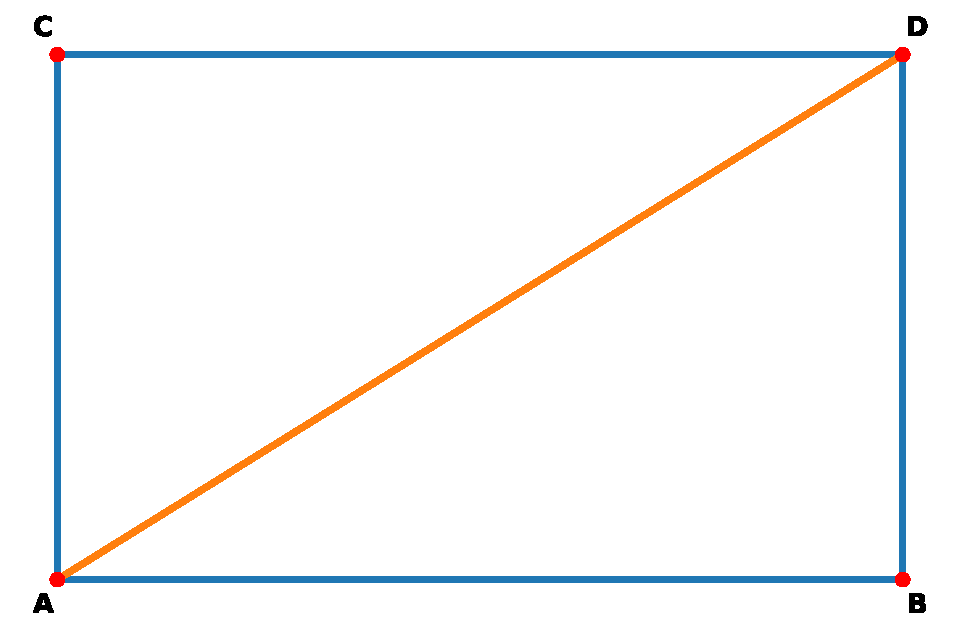
\includegraphics[width=0.5\textwidth]{rect.pdf}
\end{figure}

Notice that parallel segments $\overline{AC}$ and $\overline{BD}$ are equal in length. Likewise, $\overline{AB}$ and $\overline{CD}$ are also equal in length. $\overline{AD}$ divides the rectangle into two right triangles. By \textbf{3.2.3} we know that the two right triangles are congruent by our assertion that parallel segments of a rectangle are equal in length. Assuming that area of a rectangle is $\overline{AB}~\overline{AC}$, we can say that\medskip

\thm{}{The area of a right triangle is given by $\frac{ab}{2}$ where $a$ and $b$ are the legs of the right triangle.
}


\newpage

\chapter{Solutions}

\newpage

\section{Numbers}
\as{}{\textbf{(a.)} Prove that if $x$ is even, then $x^2$ is even\\
$x=2n$, $n \in \mathbb{Z}$\\
$x^2=4n^2$\\
$x^2=2(2n^2)$\\
\textbf{(b.)} Prove that the converse it also true\\
Suppose $x$ is not even, then $x$ is odd.
$x^2 = (2n+1)(2n+1)$ for $n \in \mathbb{Z}$\\
$x^2=4n^2+4n+1$\\
$x^2=2(2n^2+2n)+1$\\
which contradicts our assertion that $x^2$ is odd. Therefore $x$ must be even.\medskip\\
\textit{Note} that a direct way of proving (b.) would required proving that the square of an even number is even.
}

\as{}{\textbf{(a.)} Prove that if $x$ is odd, then $x^3$ is odd\\
$x=2n+1$, $n \in \mathbb{Z}$\\
$x^3=(2n+1)(2n+1)(2n+1)$\\
$x^3=8n^3+12n^2+6n+1$\\
$x^3=2(4n^3+6n^2+3n)+1$\\
\textbf{(b.)} Prove that the converse is also true\\
Suppose that $x$ is even\\
$x^3=(2n)(2n)(2n)$ for some $n \in \mathbb{Z}$\\
$x^3=8n^3=2(4n^3)$\\
But we asserted that $x^3$ is odd, therefore we were wrong to assume that $x$ is even.
}

\as{}{\textbf{(a.)} Prove that the sum of two even numbers is even\\
$2n + 2m = 2k$, $n, m, k \in \mathbb{Z}$\\
$2(n+m) = 2k$ let $n+m=k$\\
\textbf{(b.)} Prove that the sum of two odd numbers is also even\\
$(2n+1) + (2m+1) = 2k$, $n, m , k, \in \mathbb{Z}$\\
$2(n+\frac{1}{2}) + 2(m+\frac{1}{2})=2k$\\
$2(n+m+1)=2k$
}

\as{}{$x$ and $y$ are positive real numbers. If $x < y$ then show that $x^2 < y^2$\\
Suppose that $x^2 \geq y^2$ then\\
$y^2-x^2\leq0$\\
$(y+x)(y-x)\leq0$ \hspace{25pt} \textit{Note:} $(y-x)\geq0$ because $x < y$\\
We get that $y\leq x$ and $y \leq -x$ which is a contradiction because $y > x$ and $y$ is positive
}

\as{}{Given $a, b, c \in \mathbb Z$, if $a^2 | b$ and $b^3 | c$ show that $a^6 | c$\\
$b=a^2n$\\
$c=b^3m$\\
$c=(a^2n)^3m$\\
$c=a^6n^3m$
}

\as{}{Given $a, b, c \in \mathbb{Z}$, if $b|a^2$ and $c|b^3$ show that $c|a^6$\\
$a^2 = bn$\\
$b^3 = cm$\\
$b=\frac{a^2}{n}$\\
$\frac{a^6}{n^3}=cm$\\
$a^6=cmn^3$
}

\as{}{Show that $2n \choose n$ is even for all whole numbers $n$\\
$|M|=2n$\\
$\forall X_i \subseteq M$ where $|X_i|=n$, $|M-X_i|=2n-n=n$\\
For each $X_i$, there is a corresponding $X_j$ where $X_i \cap X_j=\{\}$.
Therefore, the amount of subsets of $M$ must be even.
}

\as{}{Show that $\sqrt{2}$ is irrational\\
Suppose that $\sqrt{2}$ is rational, then $\sqrt{2}=\frac{a}{b}$ for some integers $a$ and $b$.\\
Since all rational numbers have the property that $a$ and $b$ cannot share a common factor, we can assume that $\frac{a}{b}$ is reduced.\\
$\sqrt{2}b=a$\\
$2b^2=a^2$ it was proven that $a$ is even in an earlier \textit{lemma}.\\
So, $a=2n$ for some $n \in \mathbb{Z}$\\
$b^2=2n^2$.\\
Since $a$ and $b$ are both even, they share a common factor\textendash which is a contradiction because all fractions can be represented in reduced form. So $\sqrt{2}$ must be irrational.
}

\as{}{Prove that $n!$ is always even if $n>1$\\
The product of two even numbers is even:\\
$(2n)(2k)$\\
$2(nk)$\\
The product of an even number and an odd number is even:\\
$(2n)(2k+1)$\\
$4nk+2n$\\
$2(2nk+n)$\\
Since the factors of $n!$ has at least one even number, $n!$ is even.
}



%Just extra stuff ignore this lol
\nt{To know whether the usage of an \textit{or} statement is exclusive or inclusive, decide if the text explicitly uses words like ``either'' that may denote exclucivity. Second, see if both propositions can be true at the same time. If they cannot both be true, then the statement must \textit{exclusive or}, denoted symbolically as $\veebar$.}

\end{document}
